\chapter{Adattamento a nuove altitudini}
	Dopo aver cercato di stimare, nei Capitoli precedenti, la minima rete neurale in grado di effettuare le previsioni delle maree, analizzando il problema sotto vari aspetti, entreremo adesso più nel dettaglio del problema, tentando di costruire un modello sempre più accurato della rete neurale della \textit{Cerithidea Decollata}.\\
	\\
	Nello specifico, in questo Capitolo tenteremo di riprodurre un esperimento condotto dal Prof. Vannini, nel quale degli esemplari di \textit{Cherithidea Decollata}, residenti ad una determinata altitudine, vengono traslocati ad una nuova altitudine (in questo caso, più bassa dell'iniziale), per poter studiare come le chiocciole si adattano alla nuova situazione.\\
	\\
	Innanzitutto, sono state apportate delle modifiche al modello definito nei precedenti Capitoli. Le osservazioni consistono adesso nell'osservare soltanto l'arrivo della marea (ovvero, quando questa supera il livello del terreno) e arrivo ed altezza del picco di marea. L'osservazione del riflusso della marea è stato eliminato, in quanto informazione ridondante conoscendo le prime due informazioni. Inoltre, quando queste chiocciole sono salite sul tronco e si sono ancorate, entrano in una specie di sonno, rendendo quindi improbabile l'osservazione del riflusso di marea. È stata inoltre introdotta una memoria per le chiocciole, della durata di circa 28 giorni (ovvero un interno ciclo di marea), e la possibilità di utilizzare o meno un orologio lunare, che aiuti le chiocciole nella previsione.\\
	È stata quindi utilizzata una rete neurale di tipo \textit{feed-forward} (come visto nei Capitoli precedenti, un Multilayer Perceptron) con \textbf{8 neuroni} nello strato nascosto, inizialmente addestrata su un insieme di informazioni relative all'altitudine iniziale, fissata ad \textbf{1.5} (con 2 massimo picco di marea, 0 livello del mare e -2 massimo riflusso di marea). Quindi, le chiocciole vengono ``traslocate'' alla nuova altitudine, fissata a \textbf{0.5}, e vengono addestrate con le nuove informazioni, suddividendo l'addestramento in giorni. Ogni giorno, vengono fatte \textit{4 osservazioni} di marea, durante le quali le chiocciole modificheranno la propria rete neurale fino a trovare un riscontro con le informazioni appena acquisite e con le informazioni che hanno ancora in memoria. Quindi viene aggiornata la memoria della chiocciola, eliminando le 4 osservazioni più vecchie ed inserendo le 4 osservazioni appena eseguite. Infine, viene calcolato l'errore che la chiocciola commetterà prevedendo la marea nel giorno corrente e nei \textbf{27 giorni} successivi (si veda il parametro \lstinline{validationDays}, del Codice \ref{lst:tideFF_adapt}). Questo procedimento viene reiterato per più giorni finché l'errore commesso nel giorno corrente e nei 27 successivi (ovvero, per un intero ciclo di marea) non risulta essere minore di un valore prefissato (vedi parametro \lstinline{errPerc}), in questo caso il \textbf{5\%}.\\
	Eseguendo quindi una serie di test con i parametri appena elencati è risultato che le chiocciole si adattano alla nuova altitudine in circa \textbf{9 giorni} di addestramento. Non è quindi necessario che esse osservino l'intero ciclo di marea nella nuova condizione per poter prevedere la marea con un errore medio inferiore al \textbf{5\%}.\\
	\\
	Si è introdotto anche un orologio lunare, in questo modello, per studiare come cambiano le previsioni quando le chiocciole sono in possesso di quest'informazione aggiuntiva. I risultati sono stati piuttosto deludenti: se viene utilizzato soltanto l'orologio lunare, le chiocciole non riescono ad adattarsi alla nuova altitudine entro l'errore prefissato; se utilizzato in concomitanza con l'osservazione diretta della marea, non sono stati registrati risultati degni di nota: nella maggior parte dei casi si hanno differenze di un solo giorno, o anche nessuno, per quanto riguarda l'addestramento.\\
	Un'osservazione degna di nota riguarda invece il fatto che, aumentando il numero di neuroni della rete neurale, i giorni necessari per l'adattamento aumentano. Questo è dovuto al fatto che un maggior numero di neuroni implica una maggior complessità della rete neurale e di conseguenza un numero maggiore di giorni necessari per l'adattamento. Questo risultato non fa altro che evidenziare, ancora una volta, che la rete neurale necessaria per questo tipo di previsioni è estremamente semplice.\\
	\\
	Vediamo di seguito due previsioni all'altitudine iniziale\\
	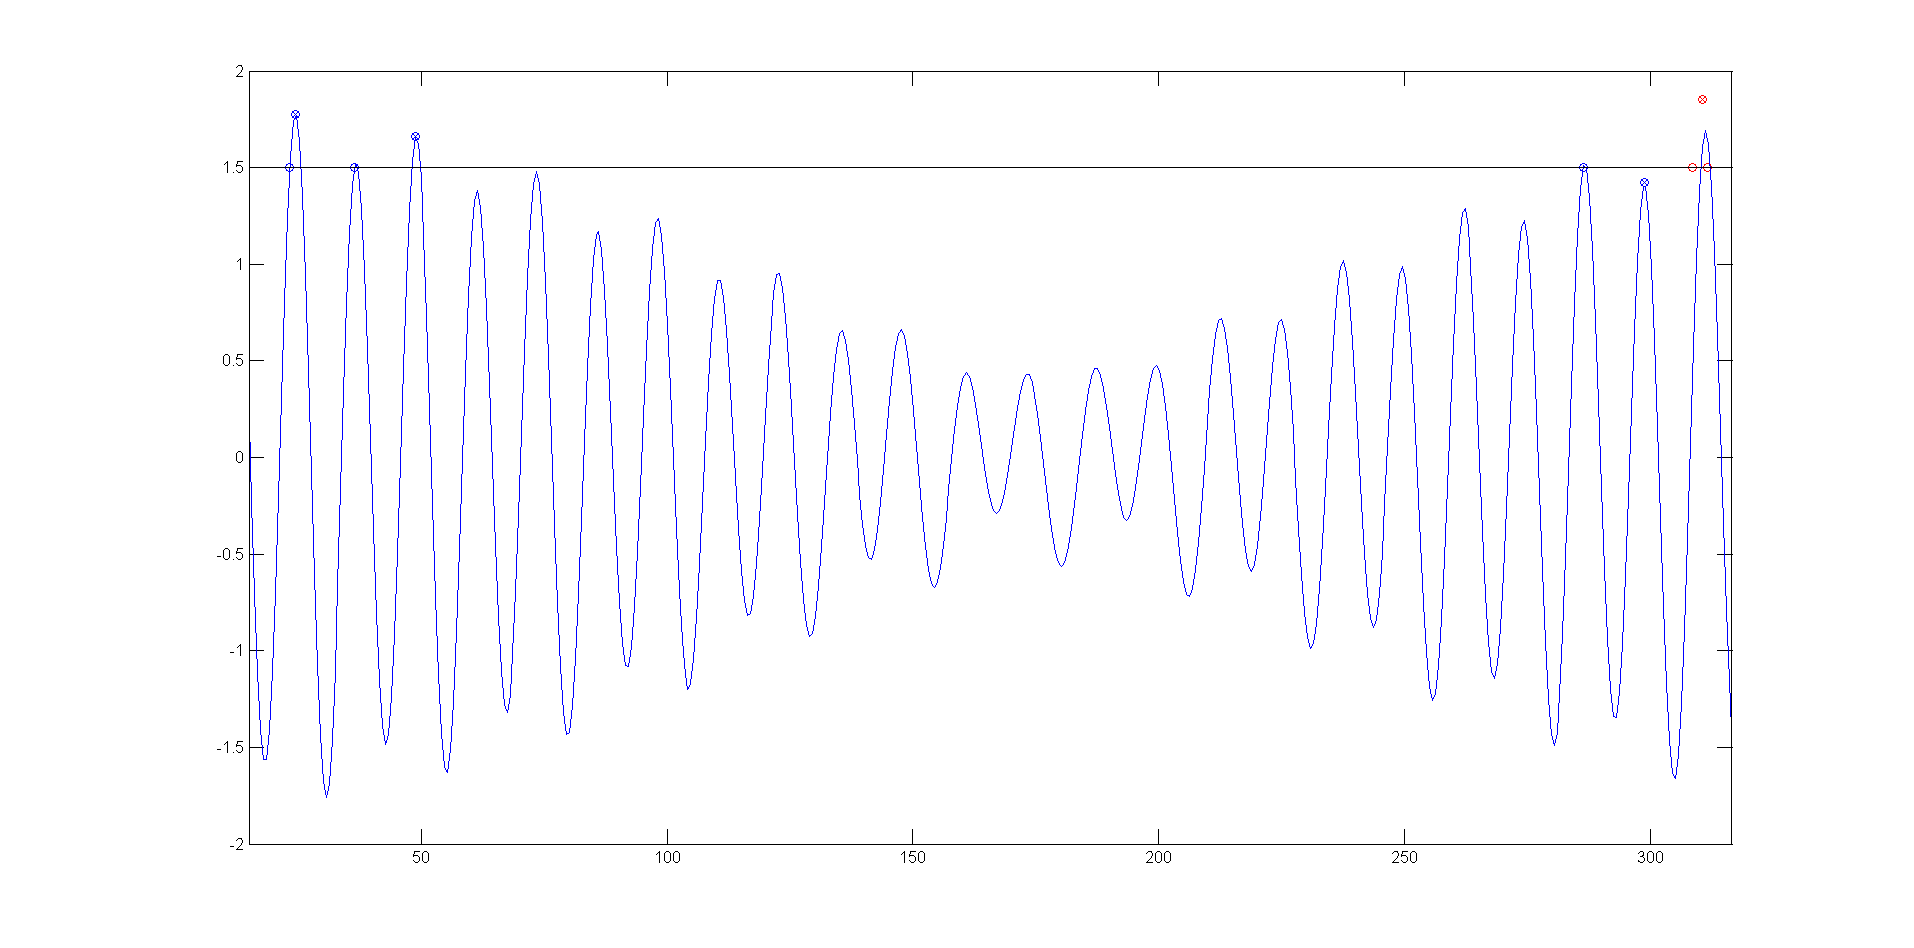
\includegraphics[width=0.5\textwidth]{adapt1_a.png}
	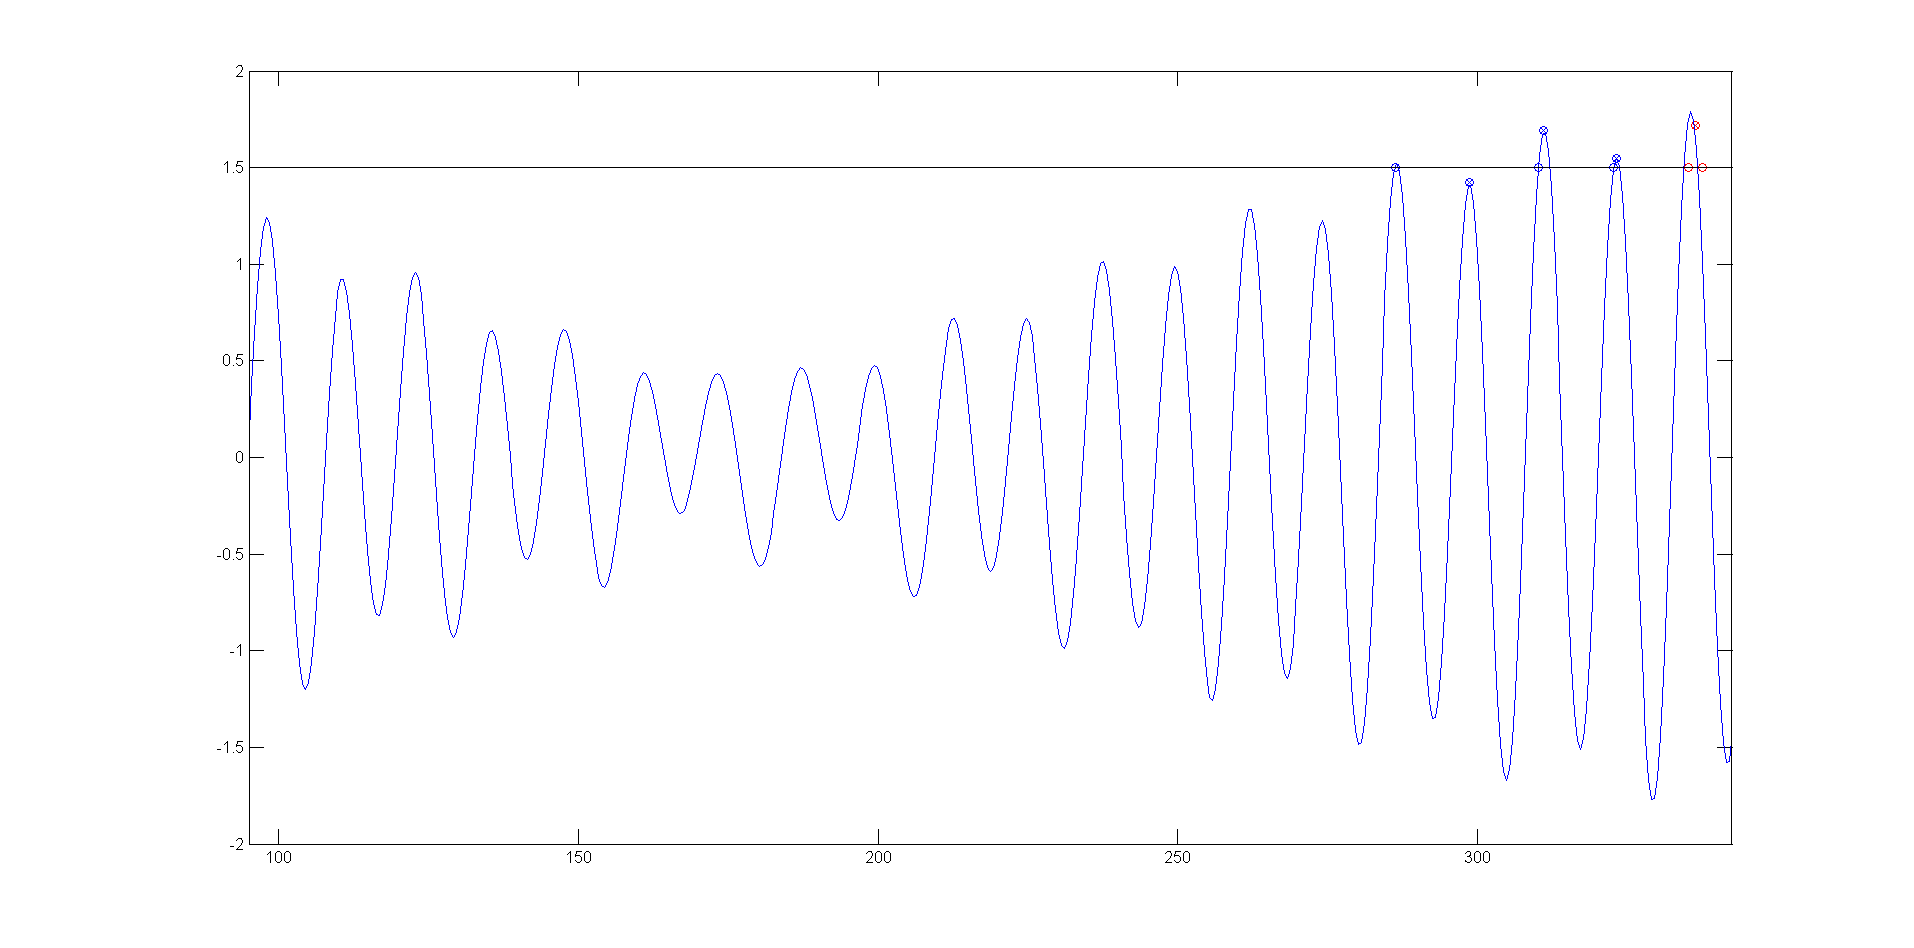
\includegraphics[width=0.5\textwidth]{adapt1_b.png}
	e due previsioni alla nuova altitudine dopo l'addestramento\\
	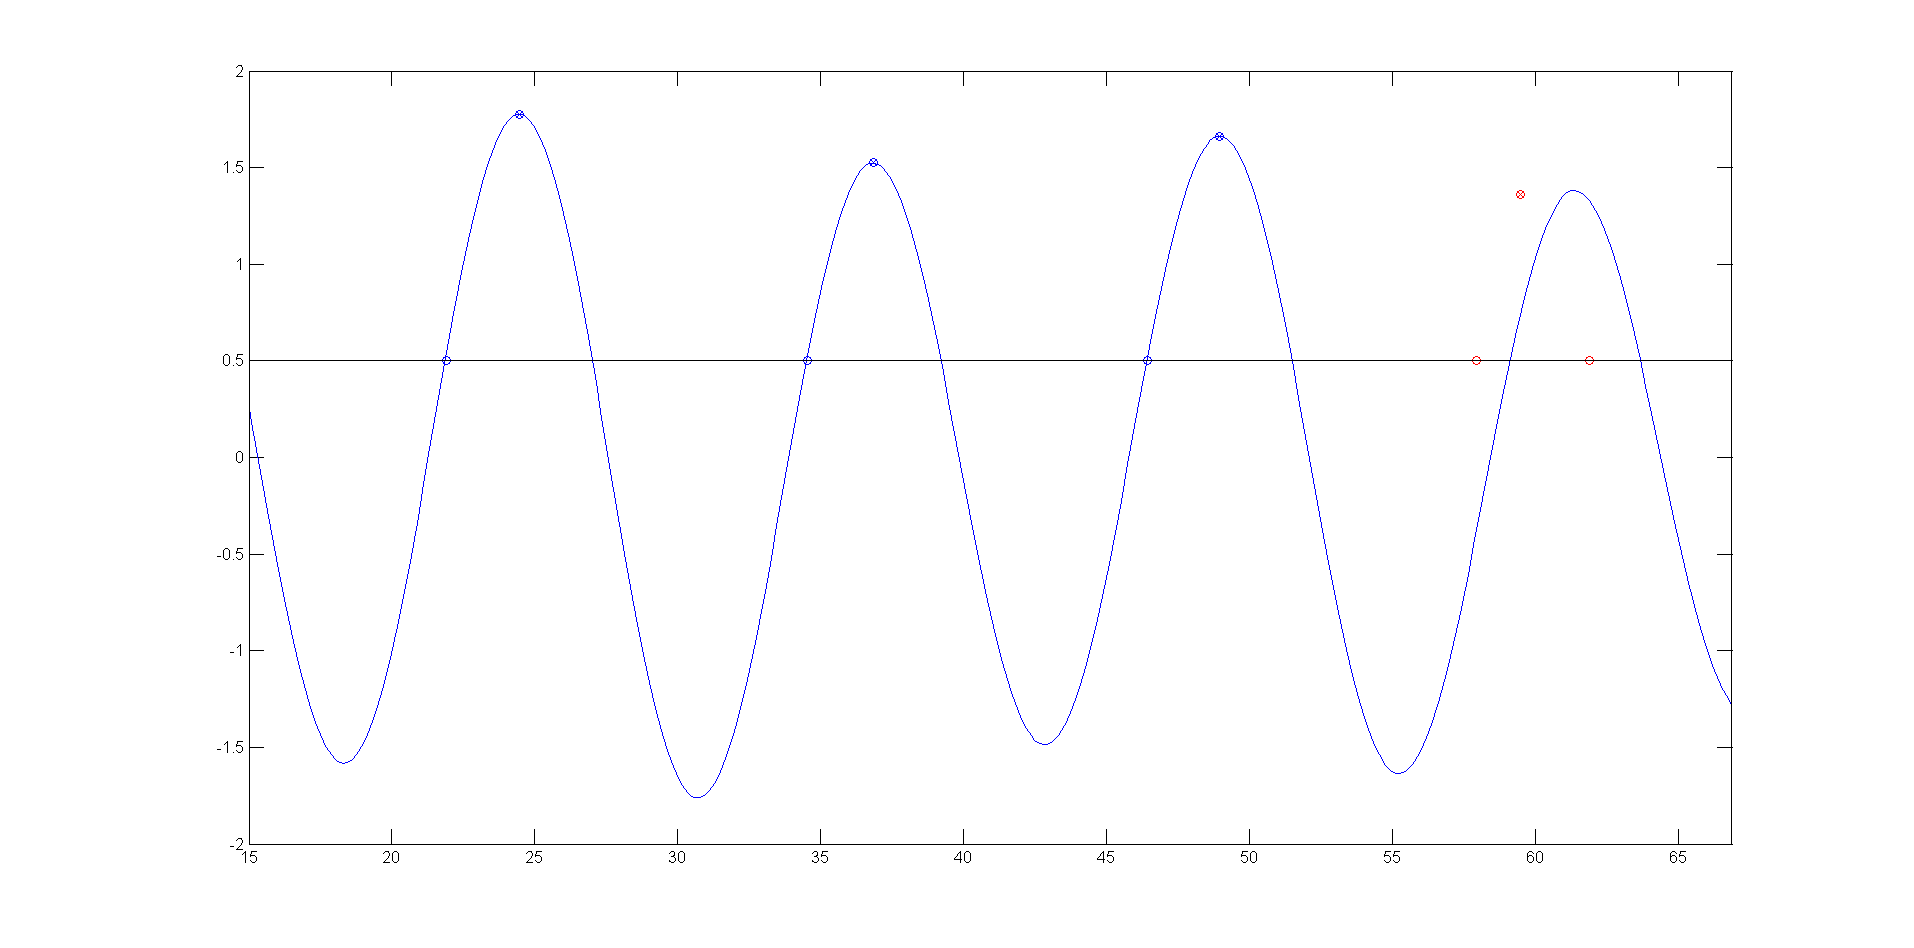
\includegraphics[width=0.5\textwidth]{adapt2_a.png}
	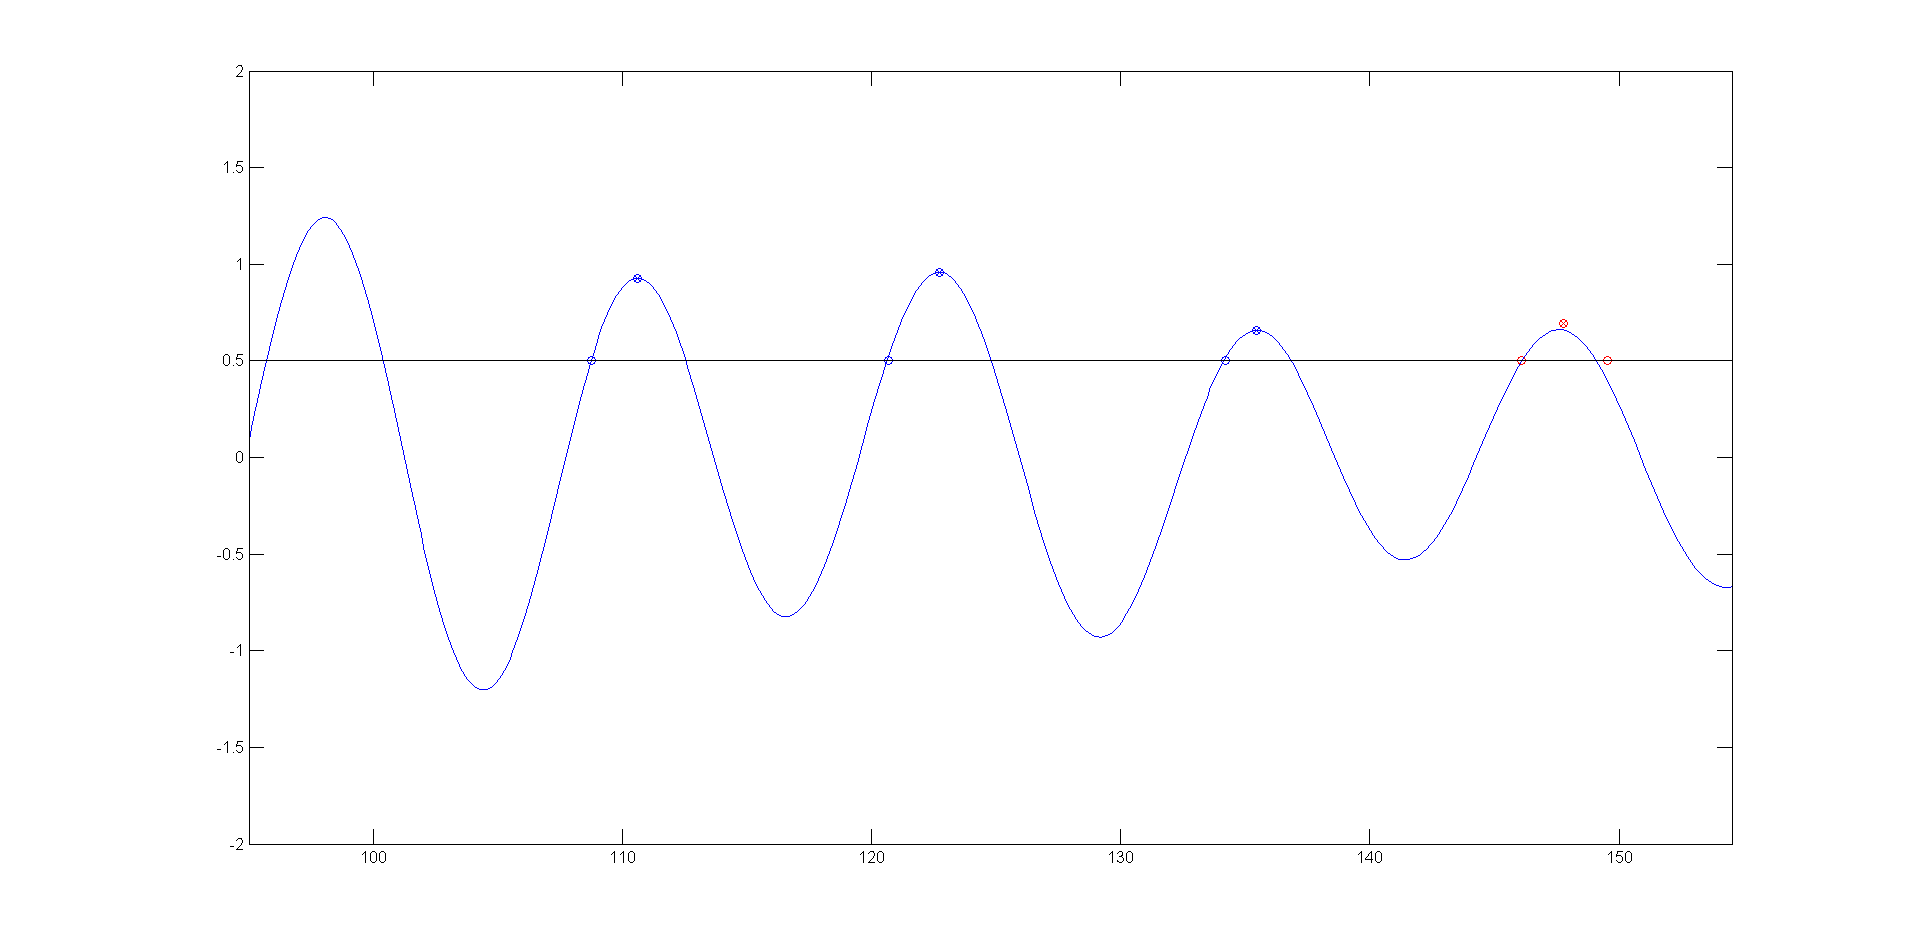
\includegraphics[width=0.5\textwidth]{adapt2_b.png}
	Il Codice \textsc{Matlab} utilizzato per queste simulazioni è il Codice \ref{lst:tideFF_adapt}, Listato del codice.